\documentclass{doctoral}

\usepackage[T1]{fontenc}
\usepackage[export]{adjustbox} % multipanels
\usepackage{bm}
\usepackage{tikz}
\usepackage{xcolor}
\usepackage{indentfirst}
\usepackage{apptools}


% Mathematical symbol abbreviations
\newcommand{\pd}{\partial}
\newcommand{\dd}{\mathrm{d}}
\newcommand{\Reynolds}{\mathrm{Re}}
\newcommand{\mm}[1]{\bm{\mathsf{#1}}} % for typesetting matrices

% Display names of python packages
\newcommand{\code}[1]{\texttt{\detokenize{#1}}}

% Gray out sections
\newcommand{\grayout}[1]{{\leavevmode\color{gray}#1}}

% For faster compilation
% Redefine \includepdf to print its arguments rather than include pages
\renewcommand{\includepdf}[2][]{\clearpage\par\texttt{\string\includepdf} arguments: \detokenize{#2}\par\clearpage}

\title{Hydrodynamic techniques\\in the study of elastic macromolecules}
\author{Radost Waszkiewicz}
\supervisor{dr hab. Maciej Lisicki, prof. UW}
\affiliation{University of Warsaw\\Faculty of Physics}

\addbibresource{sources.bib}

\begin{document}
\maketitle
\sortcitefirst{Waszkiewicz_2021_hydrodynamic, Waszkiewicz_2021_stability, Waszkiewicz_2023_dna, Waszkiewicz_2023_pychastic, Waszkiewicz_2024_mda, Waszkiewicz_2024_trimer}

\section*{Summary}

Recent, increasingly accurate measurements of the properties of bio-relevant molecules challenge our understanding of macromolecules as having well-defined, fixed shapes that determine their function.
The equilibrium distribution of their conformations is described by the Boltzmann distribution, which combines two terms: the influence of the temperature of the solvent and the potential energy of a given configuration which in turn, captures the elastic properties of the molecules.
The behavior of elastic macromolecules is thus shaped by the competition of these two physical phenomena -- whenever the valleys of the potential energy landscape are shallow in comparison to a typical thermal fluctuation, a wide variety of conformations are present; conversely, when they are deep, only small deviations from the energy-minimizing configurations can be observed.

The doctoral thesis presents a theoretical description of conformational variability of elastic macromolecules and its effect on diffusion.
The first part of the thesis provides an overview of theoretical fundamentals required for building coarse-grained models, which form the core of this work.
It also delves into the theoretical underpinnings of the experimental methods used to validate simplifying assumptions made in the former.

The second part of the thesis comprises a series of thematically linked publications and preprints in which we demonstrate methods for dealing with, and taking advantage of, both extremes of the elasticity spectrum.

Starting from molecules with very large persistence length compared to their size, we demonstrate how to model the approach of a very short DNA segment towards a nanopore and provide an analysis of the influence of wall interaction and hydrodynamic anisotropy in the nanopore capture process.
We establish theoretical criteria for determining when and where inclusion of wall corrections is necessary by considering a rod-like molecule with uniformly distributed charge.
Secondly, we investigate the impact of negative supercoiling and curvature on the hydrodynamic properties of 336 bp and 672 bp DNA minicircles.
Utilizing linear elasticity theory and hydrodynamic calculations, we predict DNA shapes and diffusion coefficients.
Our results show favorable comparison with experimental data of diffusion and sedimentation coefficients obtained using analytical ultracentrifugation.

For intermediate values of persistence length, we determine the range of lengths and g-forces under which sedimentation of a flexible, looped filament remains stable to buckling.
Our analysis, based on linear elasticity theory combined with resistive force theory, yields a stability criterion reliant on a single dimensionless parameter.

In a more general case where both thermal fluctuations and elastic forces are significant, we propose a numerical approach.
This approach is based on a stochastic differential equations integrator we developed, combined with hydrodynamic interactions based on the Rotne-Prager approximation.
Additionally, we present a suite of Python packages designed to make small Brownian Dynamics simulations both fast to develop and fast to simulate, thanks to hardware acceleration.

We deomnstrate that for the intrinsically disordered proteins (IDPs), which represent the opposite extreme of the elasticity spectrum as compared to very stiff DNA, excluded volume interactions are the key factor determining the equilibirum conformational ensemble.
Introducing the Globule-Linker model of conformations and we combine it with the Minimum Dissipation Approximation to predict their hydrodynamic size.
Using the comparison of the coarse grained approach with the largest set of experimental valeus to date, we show that our first principles approach outperforms phenomenological fits available in the literature.

Finally, we deal with a theoretical problem of equilibrium distributions of molecules with both very stiff degrees of freedom and comparatively free ones (such as bond length and inter-bond angles respectively).
We identify important details of the constraining potentials overlooked in the earlier works and demonstrate a method for their computation, both in general and through specific examples.

Our results, spanning a spectrum of possible elastohydrodynamic regimes, demonstrate the rich diversity of phenomena arising from the competition of structural rigidity and viscous stresses.
In order to facilitate the analysis of such systems, we have created a number of open source numerical tools, which have been published with documentation.
The applicability of these tools was tested directly in relatively stiff biopolymer -- the DNA -- and soft strucures of IDPs.
Additionally, they provide an insight into the intermediate stiffness regimes, where thermal fluctuations compete with intramolecular interactions, and can be used for a better understanding of microscale elastohydrodynamic phenomena.
\clearpage

\section*{Streszczenie}
Nowe, coraz dokładniejsze pomiary właściwości istotnych biologicznie cząsteczek podważają nasze rozumienie makromolekuł jako cząsteczek o dobrze określonych, stałych kształtach określających ich funkcję.
Rozkład równowagowy ich konformacji opisuje rozkład Boltzmanna, który łączy w sobie następujące dwa człony: wpływ temperatury rozpuszczalnika oraz energię potencjalną danej konfiguracji, która z kolei opisuje właściwości elastyczne danej cząsteczki.
Zachowanie elastycznych makromolekuł jest zatem kształtowane przez konkurencję tych dwóch zjawisk fizycznych -- gdy studnie potencjału są płytkie w porównaniu z typowymi fluktuacjami termicznymi, występuje szeroka gama konformacji; i odwrotnie, gdy są głębokie, można zaobserwować jedynie niewielkie odchylenia od konfiguracji minimalizujących energię.

W niniejszej rozprawie doktorskiej przedstawiono teoretyczny opis zmienności konformacyjnej elastycznych makromolekuł i jej wpływu na ich dyfuzję.
Pierwsza część rozprawy zawiera przegląd podstaw teoretycznych wymaganych do budowy modeli gruboziarnistych, które stanowią istotę rozprawy oraz teoretyczne podstawy metod eksperymentalnych stosowanych do weryfikacji założeń upraszczających owych modeli.
Druga część rozprawy składa się z szeregu powiązanych tematycznie publikacji i preprintów, w których prezentujemy metody modelowania molekuł w szerokim spektrum sprężystości.

Zaczynając od cząsteczek o dalekim zasięgu korelacji elastycznych (ang. persistence length) w porównaniu z ich rozmiarem, pokazujemy jak modelować zbliżanie bardzo krótkiego segmentu DNA do nanoporu i analizujemy wpływ ścian i anizotropii hydrodynamicznej w procesie wychwytywania cząstek przez nanopory.
Ustalamy teoretyczne kryteria tego, w jakich przypadkach konieczne jest uwzględnienie oddziaływania cząsteczek ze ściankami, przybliżając molekuły przez pręt z równomiernie rozłożonym ładunkiem elektrycznym.
Ponadto, badamy wpływ ujemnego trzeciorzędowego skręcenia (ang. supercoiling) i krzywizny DNA na właściwości hydrodynamiczne mini-pętli DNA o długości 336 bp i 672 bp.
Wykorzystując liniową teorię elastyczności i modelowanie hydrodynamiczne, przewidujemy kształty DNA i ich współczynniki dyfuzji.
Dane eksperymentalne współczynników dyfuzji i sedymentacji uzyskane za pomocą ultrawirowania analitycznego pokazują dobrą zgodność z naszymi przewidywaniami teoretycznymi.

Dla pośrednich wartości zasięgu korelacji elastycznych wyznaczamy taki zakres długości i sił zewnętrznych, przy którym sedymentacja elastycznej, cienkiej pętli pozostaje stabilna na wyboczenia.
Nasza analiza, oparta na liniowej teorii elastyczności połączonej z lokalnym oporem hydrodynamicznym, wyznacza kryterium stabilności zależne od pojedynczego bezwymiarowego parametru.

W bardziej ogólnym przypadku, gdy istotne są zarówno fluktuacje termiczne, jak i siły sprężyste, prezentujemy podejście numeryczne.
Nasze podejście opiera się na algorytmie całkowania stochastycznych równań różniczkowych połączonym z oddziaływaniami hydrodynamicznymi opartymi na przybliżeniu Rotne-Pragera.
Powyższe metody zostały udostępnione jako zbiór paczek w Pythonie zaprojektowanych w celu szybkiego programowania i przeliczania małych symulacji dynamiki Browna.

W przypadku białek nieustrukturyzowanych (ang. IDP), które reprezentują przeciwną skrajność elastyczności w porównaniu z bardzo sztywnym DNA, objętość wykluczona jest determinantą dystrybucji w rozkładach równowagowych.
Przedstawiamy model konformacji Globule-Linker, który w połączeniu z Przybliżeniem Minimalnej Dyssypacji pozwala obliczyć wielkość hydrodynamiczną takich białek.
Porównując podejście gruboziarniste z największym jak dotąd zmierzonym zbiorem danych eksperymentalnych, pokazujemy, że nasze podejście umocowane w prawach fizycznych jest skuteczniejsze niż dopasowania fenomenologiczne dostępne w literaturze.

W ostatnim artykule rozważamy teoretyczny problem rozkładów równowagowych cząsteczek o wielu stopniach swobody z których część jest silnie związana (jak na przykład długości wiązań chemicznych).
Pokazujemy, że istotne detale potencjałów realizujących więzy zostały przeoczone we wcześniejszych pracach oraz proponujemy właściwą metodę ich uwzględnienia.

Nasze wyniki, obejmujące szeroki zakres korelacji elastycznych, pokazują różnorodność zjawisk wynikających z współwystępowania elastyczności i fluktuacji termicznych.
Aby ułatwić analizę takich układów, stworzyliśmy zbiór otwartych narzędzi numerycznych, które zostały opublikowane wraz z dokumentacją.
Możliwość zastosowania powyższych narzędzi przetestowano bezpośrednio w stosunkowo sztywnym biopolimerze (DNA) i w miękkich strukturach (IDP).
Przedstawione narzędzia zapewniają wgląd w pośrednie reżimy sztywności, w których fluktuacje termiczne konkurują z interakcjami wewnątrzcząsteczkowymi i mogą posłużyć do lepszego zrozumienia zjawisk elastohydrodynamicznych w mikroskali.

\clearpage

\section*{Manuscripts comprising this thesis}

\begin{itemize}
    \item \fullcite{Waszkiewicz_2021_hydrodynamic}
    \item \fullcite{Waszkiewicz_2021_stability}
    \item \fullcite{Waszkiewicz_2023_dna}
    \item \fullcite{Waszkiewicz_2023_pychastic}
    \item \fullcite{Waszkiewicz_2024_mda}
    \item \fullcite{Waszkiewicz_2024_trimer}
\end{itemize}

\vspace*{\fill}

\section*{Funding}
Research on the topic of the Thesis was supported by the grant \emph{Dynamic deformations of elastic filaments in viscous flows}, financed by the National Centre of Science in Poland under the grant agreement to Maciej Lisicki no.
2018/31/D/ST3/02408
\clearpage

\tableofcontents

\chapter{Introduction}

\section{Mesoscopic world of macromolecules}

A fundamental technique for assessing the relative importance of different physical mechanisms within a theoretical framework, originating in the domain of fluid mechanics (cf.
Reynolds, \cite{Reynolds_1883}), involves the consideration of dimensionless numbers.
Here, we follow the approach of Nagele \cite{Nagele_2013}, where he motivates common approximations in colloidal physics by considering timescale ratios.

Colloidal hydrodynamics focuses on the properties of colloidal suspensions, which are mixtures of very small objects (with sizes of the order of $0.1 \mathrm{\mu m}$) and a solvent, typically water.
At human-length scale, water is easily treated as incompressible (for example, by considering volume changes at typical pressures on the order of atmospheric pressure).
However, this becomes less obvious at the microscopic length scale where the granularity of matter becomes significant.
The relevant bulk density relaxation timescale $\tau_s$ at the length scales relevant to the colloidal object of size $a$ can be estimated from the speed of sound in water, $c$, as $\tau_s = a/c \approx 6 \times 10^{-11} \mathrm{s}$, which is much shorter than any experimentally relevant timescale, prompting us to use the incompressible Navier-Stokes equations.

For a Newtonian fluid (such as water) of density $\rho$ and viscosity $\eta$, these equations describe the evolution of the velocity field $\bm{u}$ in response to the pressure gradient $\bm{\nabla} p$ and body forces $\bm{f}$ acting on the fluid as
\begin{eqnarray}
    \rho \left( \frac{\pd \bm{u}}{\pd t} + \bm{u} \cdot \bm{\nabla u} \right) = - \bm{\nabla} p + \eta \Delta \bm{u} + \bm{f}, \label{eqn:navier-stokes-equation}
\end{eqnarray}
together with the incompressible continuity equation
\begin{equation}
    \nabla \cdot \bm{u} = 0 \label{eqn:incompressibility}.
\end{equation}

The Navier-Stokes equation \eqref{eqn:navier-stokes-equation} is famously nonlinear and further simplifications are necessary for almost any problem of practical relevance.
The relative importance of the nonlinear momentum advection term compared to the viscous dissipation term is measured by the Reynolds number $\Reynolds$\cite{Reynolds_1883}.
In quiescent fluid, it can be estimated from the velocity of a colloidal particle $V_p$ as
\begin{equation}
    \Reynolds = \frac{|\rho \bm{u} \cdot \bm{\nabla}\bm{u}|}{|\eta \Delta \bm{u}|} \sim \frac{\rho V_p L}{\eta}.
    \label{eqn:reynolds-based-estimate}
\end{equation}

Taking $a = 100$ \AA{} and $V_p \approx 1 \mathrm{\mu m / s}$  we get $\Reynolds \sim 10^{-7}$.
%for a particle of mass $M = 100 \mathrm{k Da}$ and $V_p$ as determined from equipartition of energy ($V_p = \sqrt{2 k_{B} T / M} \approx 7 \mathrm{m/s}$, where $k_B$ is the Boltzman constant) at room temperature $T$ 
Thus, we can disregard the nonlinear terms and arrive at the time-dependent Stokes equation
\begin{equation}
    \rho \frac{\pd \bm{u}}{\pd t} = - \bm{\nabla} p + \eta \Delta \bm{u} + \bm{f}.
    \label{eqn:time-dependent-stokes-equation}
\end{equation}

By taking curl of both sides of this equation, we arrive at the vorticity diffusion equation, for vorticity $\omega = \bm{\nabla} \times u$
\begin{equation}
    \frac{\pd}{\pd t} \bm{\omega}  = \frac{\eta}{\rho} \Delta \bm{\omega} , \label{eqn:vorticity-diffusion}
\end{equation}
which has a heat-kernel-type solution with characteristic time of
\begin{equation}
    \tau_\omega = \frac{\rho a^2}{\eta}.
    \label{eqn:vorticity-timescale}
\end{equation}

It turns out that this timescale is of the same order as the Rayleigh particle velocity relaxation timescale $\tau_B$ (following the naming convention of \textcite{vanKampen_2011}) describing the exponential decay of the velocity of a solid particle of radius $a$ slowing down due to Stokes drag $F_{stokes} = 6 \pi \eta a V_p = \zeta V_p$ as shown by
\begin{equation}
    \tau_B = \frac{M}{\zeta} = \frac{2}{9} \left( \frac{\rho_p}{\rho} \right) \tau_\omega, \label{eqn:raighley-timescale}
\end{equation}
where $\rho_p$ is the density of the colloidal particle, which is often neutrally buoyant.

Finally we can define the diffusive timescale $\tau_D$ as the time required for a particle to move distance comparable with its size while diffusing with coefficient of diffusion $D$
\begin{equation}
    \tau_D = \frac{a^2}{D}.
    \label{eqn:diffusive-timescale}
\end{equation}

Thus for colloidal particles $\tau_D \gg \tau_\omega \sim \tau_B$ and on experimentally relevant time scales $\sim \tau_D$ we can neglect time dependent terms of the Stokes equation (this is not always the case, for example in the motion of carpets of cilia or bacterial flagella the time dependent terms play a role \cite{Wei_2021}).
Consequently, we arrive at the Stokes equations
\begin{eqnarray}
    \eta \Delta \bm{u} - \bm{\nabla} p + \bm{f} = 0, \label{eqn:stokes-equation} \\
    \nabla \cdot \bm{u} = 0.
\end{eqnarray}

The Stokes equation \eqref{eqn:stokes-equation} possesses important properties of linearity and instantaneous information propagation throughout the domain.
This means that the velocity at any moment is fully determined by the fluid boundary conditions at the same time instance.
These properties are vital for the construction of mobility matrices discussed in the next section.

\section{Mobility matrices}

An immediate corollary of the linearity of the Stokes equation is the existence of so-called mobility matrices -- linear operators that provide particle velocities resulting from forces and torques acting within a given configuration of colloidal particles.
Unfortunately, closed-form expressions for these relationships exist only in very simple geometries where flows can be easily computed, such as for a single sphere or ellipsoid.
Even for highly symmetric shapes, such as a torus \cite{Goren_1980, Majumdar_1977}, solutions are, at best, expressed in terms of a series expansion.
We can leverage the very simple solution for flow around a sphere and construct an approximate solution for flow around multiple spheres.
In this manner, we can model many bodies of interest in a modular fashion by approximating them as a collection of small spheres, connected either rigidly or through appropriate potentials.
This construction is facilitated by the method of mobility matrices, which we describe below.

Consider $N$ spherical particles each of radius $a$ located at $\bm{R}_i$ for $i \in (1 \dots N)$ moving with velocities $\bm{V}_i$ and angular velocities $\bm{\Omega}_i$ under the influcence of external forces $\bm{F}_i$ and torques $\bm{T}_i$.
We seek the matrix connecting these velocties to these forces.
For convenience this section uses supervector notation, here following convention of \cite{Nagele_2013}.
Let us denote a concatenated vector of particle velocities as $\bm{V} = (\bm{V}_1,\bm{V}_2,\dots,\bm{V}_N)^{T}$, angular velocities and $\bm{\Omega} = (\bm{\Omega}_1,\bm{\Omega}_2,\dots,\bm{\Omega}_N)^{T}$ and analogously for forces $\bm{F}_i$ and torques $\bm{T}_i$ 

From the linearity of the Stokes equation and the no-slip boundary conditions of the fluid velocity at the surface of the colloids we know that they obey a linear relationship.
We can introduce mobility tensors $\mm{\mu}$ in the following fashion
\begin{equation}
    \begin{pmatrix}
        \bm{V} \\
        \bm{\Omega}
    \end{pmatrix}
    = -
    \begin{pmatrix}
        \mm{\mu}^{tt} & \mm{\mu}^{tr} \\
        \mm{\mu}^{rt} & \mm{\mu}^{rr}
    \end{pmatrix}
    \cdot
    \begin{pmatrix}
        \bm{F} \\
        \bm{T}
    \end{pmatrix}
    .
    \label{eqn:mobility-matrix-definition}
\end{equation}
Often one is interested in a torque free case where only submatrix $\mm{\mu}^{tt}$ plays a role and is referred to as translational mobility matrix or grand translation mobility matrix (to emphasise that it captures particle-particle interactions).

For a point force $\bm{f}$ acting on the fluid Green's function of the Stokes equation is called the Oseen tensor $\mm{T}^0$ with fluid velocity satistying $\bm{u}(\bm{r}) = \mm{T}^{0}(\bm{r}).
    \bm{f}$.
Said tensor is given by
\begin{equation}
    \mm{T}^{0}(\bm{r}) = \frac{1}{8\pi\eta |\bm{r}|} \left( \mm{1} + \bm{\hat{r}}\bm{\hat{r}}\right).
\end{equation}

For multiple spherical colloids suspended in a quiescent fluid, the mobility matrices depend on the relative positions of the spheres.
In the lowest order approximation, it turns out that only pairwise displacements $\bm{R}_{ij} = \bm{R}_i - \bm{R}_j$ are required to compute them.
It may be tempting to simply evaluate the Oseen tensor at the centers of the spheres and use this as a mobility matrix; unfortunately, this approach can lead to a matrix that is not positive definite, which physically corresponds to negative dissipation of energy under some forcing.
As a result, this approach is not just inaccurate but completely fruitless in the case of Brownian Dynamics where square roots of mobility matrices are required at each simulation step.
Most methods for computing square roots (such as the Cholesky decomposition) are singular for singular matrices.
Thus even a very small error in the components of the mobility tensor can lead to arbitrarily large erros of the square root unless positive definiteness can be guaranteed.

Introducing $R_{ij} = |\bm{R}_{ij}|$ we can determine the velocity of $i^{th}$ sphere exactly from the surface tractions integral by combining Faxen's law \cite{Faxen_1922} with the Oseen tensor.
\begin{equation}
    \bm{V_i} =
    -\mu_0^t \bm{F}_i
    + \sum_{j\neq i}^N
    (1 + \frac{a^2}{6} \Delta_i)
    \int_{S_j} \dd S' \mm{T}^0(\bm{R}_i-\bm{r'})\cdot \bm{f}^{(s)}(\bm{r'}).
    \label{eqn:faxen-theorem}
\end{equation}

A direct use of equation \eqref{eqn:faxen-theorem} is not very practical since it requires solving for surface traction distribution.
If we only take into account the average surface traction on each sphere  by $\bm{f}_j^{(s)}(\bm{r'}) = -\bm{F}_j / (4\pi a^2)$ taking one obtains relationship of the form \eqref{eqn:mobility-matrix-definition}.
Next, one can approximate the integrand by Taylor expanding it around centres of spheres to second order (with remainder term $\mathcal{O}((a/R_i)^4)$ because the integrals of all third order terms vanish) we get lowest order in $a$ approximation of the mobility tensors 

\begin{eqnarray}
    \bm{V}_i \approx -\mu_0^t \bm{F}_i  - \sum_{j\neq i}^N (1 + \frac{a^2}{6} \Delta_i) (1 + \frac{a^2}{6} \Delta_j) \mm{T}^{0} (\bm{R}_i - \bm{R}_j) \cdot \bm{F_j} \\
    \approx -\mu_0^t \bm{F}_i  - \sum_{j\neq i}^N (1 + \frac{a^2}{3} \Delta_x) \mm{T}^{0} (\bm{x} = \bm{R}_{ij}) \cdot \bm{F}_j \label{eqn:rotne-prager-derivation}
\end{eqnarray}
because $\Delta_i \Delta_j \mm{T}^0(\bm{R}_{ij}) = 0$.
%(recall surface integrals of polynomials of order up to 2, express them in terms of surface area

Evaluating the Laplacians and rearranging the explicit formulae for mobility tensors can be obtained
\begin{eqnarray}
    \mm{\mu}_{ii}^{tt,RP} & = & \mu_0^t \mm{1},                                                                                                                                                                                                                                                                  \\
    \mm{\mu}_{ij}^{tt,RP} & = & \mu_0^t \left( \frac{3}{4} \left( \frac{a}{R_{ij}} \right) \left( \mm{1} + \bm{\hat{R}}_{ij} \bm{\hat{R}_{ij}} \right) + \frac{1}{2} \left( \frac{a}{|R_{ij}|} \right)^3 \left( \bm{1} -3  \bm{\hat{R}}_{ij}\bm{\hat{R}}_{ij} \right) \right) \quad \mathrm{for} \quad i \neq j.
    \label{eqn:rotne-prager-translation}
\end{eqnarray}

The $\mm{\mu}_{ij}^{tt,RP}$ approximation is the well known Rotne-Prager approximation \cite{Nagele_2013,Dhont_2008,Kim_2013}.
It turns out that this approximation is always positive definite thus a great candiate for Brownian dynamics applications.
Moreover, it turns out that tensor divergence of $\mm{\mu}^{tt,RP}$ is equal to zero (which is not true for the exact solution $\mm{\mu}^{tt}$) elliminating another term problematic for Brownian dynamics simulations in a self-consistent manner\cite{Ermak_1978}.
Completely analogous procedure can be applied to the $tr$ and $rr$ parts of the mobility matrix.
That and further improvements (such as differentiable continuation for overlaps) are discussed by \textcite{Zuk_2018}.

\section{Mathematical treatment of Brownian motion}
\label{sec:SDE}

Although the fundamentals of kinetic theory of gases had been established since the 1870s and Navier-Stokes equations since the 1840s, the formulation of the earliest fluctuation-dissipation-type equation, now known as the Stokes-Einstein relationship ($D = 1 / (6 \pi \eta a)$ for a spherical particle), first appeared in the contributions of Einstein \cite{Einstein_1905} and Smoluchowski \cite{Smoluchowski_1906}.
Their theoretical insights were experimentally verified by Perrin \cite{Perrin_1909}, culminating in his Nobel Prize in Physics in 1926.
The conceptual challenge of merging two formerly distinct branches of physics was further complicated by the necessity to develop new mathematical tools capable of handling random functions describing the position and velocity of Brownian particles.
The physical heuristics devised to capture the probabilistic nature of temperature were later formalized into what is now known as stochastic calculus.
The applications of stochastic calculus found utility in the economic context, where Merton and Scholes were awarded the Nobel Prize in Economics in 1997 for their development of the Black-Scholes-Merton formula for option pricing.
However, the misuse of their results by the financial industry, coupled with inadequate regulation of the derivatives sector, led to the 2008 financial crisis \cite{fcic_report}.

We outline the central complication of the stochastic calculus (second order terms in the chain rule equivalent) using a physically motivated example.
A more succinct description of this domain can also be found in \textcite{Waszkiewicz_2023_pychastic}.
For simplicity, we will again focus on just a single colloidal sphere.
In the case of isotropic diffusion in a quiescent fluid the problem is separable with each cartesian direction being independent, in this simple case we can just consider scalar velocty and displacement.
In more complex cases (single sphere near a wall, or more than one sphere, or any other shape) more care is needed because displecements in different directions are no longer independent and often also dependent on angular displacements which complicates the problem significantly.
Following the notation of \textcite{Ottinger_2012}, we will denote time dependence in subscripts such that the (time dependent) velocity of such sphere is $V_t$.
Historically $V_t$ was modelled by the Langevin equation
\begin{equation}
    M \frac{\dd V_t}{\dd t} = - \zeta V_t + F^{B}_t \label{eqn:langevin-velocity}
\end{equation}
with $F^B_t$ a time dependent force arising from the bombardment of the colloid by the water molecules.

Langevin's heuristic solution of equation \eqref{eqn:langevin-velocity} ignored the unsual stochastic properties of $F^{B}_t$, to obtain $V_t$ as a convolution of $F_t^B$ with an appropriate Green's function.
Such a convolution is a linear operator acting on (what we hope is) a Gaussian process and thus we should be able to compute variance of the velocity $\langle V_t^2 \rangle$, with $\langle \cdot \rangle$ denoting expected value by means of a double integral
\begin{equation}
    \langle V_t^2 \rangle = \frac{1}{M^2} \int_0^t \dd t' \int_0^t \dd t'' \exp\left( - \frac{\zeta}{M} (2t - t' - t'') \right) \langle F_{t'}^B F_{t''}^B \rangle.
    \label{eqn:velocity-variance-integral}
\end{equation}

Recall that the Brownian timescale is much longer than the fluid relaxation timescale $\tau_B \gg \tau_s$ and thus we postulate that the Brownian force has a singular correlation structure
\begin{equation}
    \langle F_{t'}^B F_{t''}^B \rangle = \alpha_B \delta(t'-t''), \label{eqn:white-noise-langevin}
\end{equation}
where $\delta$ deontes the Dirac delta functional.

Evaluating the integral \eqref{eqn:velocity-variance-integral} we get
\begin{equation}
    \frac{1}{2} M \langle V_t^2 \rangle = \frac{\alpha_B}{4 \zeta} \left[ 1 - \exp \left(-2\zeta \frac{t}{M} \right) \right].
    \label{eqn:velocity-variance-solution}
\end{equation}

By applying equipartition principle to the result \eqref{eqn:velocity-variance-solution} we arrive at the necessary amplitude of the Brownian fluctuations as
\begin{equation}
    \alpha_B = 2 k_B T \zeta.
    \label{eqn:fluctuation-dissipation-raighley-particle}
\end{equation}
This is a form of fluctuation-dissipation theorem \cite{van_Kampen_1984,Ottinger_2012}.

Furthermore we can heuristically go to the limit of high damping $M/\zeta \to 0$ and obtain equation for the particles position
\begin{equation}
    \frac{\dd X_t}{\dd t} = \frac{1}{\zeta} F_t^B.
    \label{eqn:langevin-position}
\end{equation}

A proper treatment of the equation \eqref{eqn:langevin-position} is possible with the help of stochastic differential equations (SDE).
First we define standard Wiener process $W_t$ as a Gaussian martingale with the following covariance structure
\begin{equation}
    \langle W_{t_1} W_{t_2} \rangle = \int_0^{t_1} \dd t' \int_0^{t_2} \dd t'' \delta(t' - t'') = \min(t_1, t_2) \label{eqn:wiener-process-definition}
\end{equation}

Note that, this time, covariance is non-singular and the usual theory of Gaussian processes is directly applicable.
Heuristically, we expect $V_t$ to be described by the following integral
\begin{equation}
    V_t = \frac{\sqrt{2 k_b T \zeta}}{M} \int_0^t \exp\left( -\zeta\frac{t - t'}{M} \right) \dd W_{t'}.
    \label{eqn:velocity-integral-sde}
\end{equation}
Unfortunately, this integral cannot be performed pathwise because $W_t$ has infinite variation in every interval, even though the issues of almost-surely nowhere differetniability of equation~\eqref{eqn:langevin-position} are avoided.
We need some generalisation of the usual integration to formalise this notion.

These integrals turn out to be formally tractable for a class of processes called non-anticipatory.
Any such process ($X_t$, say) has the property, that for any time $t$, the future increments of the Wiener process $W_{t'} - W_t$ and past values of the process $X_{t''}$ ($t'' < t < t'$) are independent variables.

We begin construction of the stochastic integral by considering non-anticipatory random step functions -- processes which are constant on finite intervals (denoted with indicator function $\mathbb{I}$) with step heights given by random variables $\widetilde{X}_{i}$ like so
\begin{equation}
    X_t = \sum_{j=1}^{n} \widetilde{X}_{j-1} \mathbb{I}(t \in [t_{j-1},t_j]).
    \label{eqn:random-step-function}
\end{equation}

For these processes the stochastic (Ito) integral is simply defined as
\begin{equation}
    \int_0^{t_{\mathrm{max}}} X_t \dd W_t = \sum_{j=1}^{n} \widetilde{X}_{j-1} (W_{t_j} - W_{t_{j-1}}).
    \label{eqn:ito-integral-step-function}
\end{equation}
There is a noticeable lack of symmetry in this expression -- we evaluate the integrand on the left end of each interval, as a result $\widetilde{X}_{j-1}$ and $W_{t_j} - W_{t_{j-1}}$ are independent variables because of the non-anticipatory nature of the process $X_t$.
This 'direction of anticipation' asymmetry plays a central role in the differences between Ito and classical calculus (and is notably absent in Stratonovich calculus).
% $X_{j-1} \perp (W_{t_j} - W_{t_{j-1}})$

Thanks to the non-anticipation property, we can immediately conclude two very useful lemmas for random step functions (which are also true for general non-anticipating processes).
First, Ito integrals are martingales
\begin{equation}
    \left< \int_0^{t_{\mathrm{max}}} X_t \dd W_t \right> = 0.
    \label{eqn:ito-integrals-are-martingales}
\end{equation}
Second, variance of an Ito integral can be computed with a standard (non stochastic) integral
\begin{equation}
    \left< \left( \int_0^{t_{\mathrm{max}}} X_t \dd W_t \right)^2 \right> = \int_{0}^{t_{\mathrm{max}}} \left< X_t^2 \right> \dd t, \label{eqn:itos-lemma}
\end{equation}
a result dubbed Ito's lemma \cite{Ito_1951}.
To complete the construction of Ito's integral, we need an appropriate limiting procedure whereby a sequence of approximating random-step-function processes is constructed and the original integral is the limit of approximating integrals.
It turns out that the correct notion of limit here is that of mean square error, and that both the approximating processes and the integral itself converge in that sense.

To show explicitly that this notion of integration is really fundamentally distinct from the usual integration, consider a famous integral $\int_0^t W_{t'} \dd W_{t'}$.
We can easily construct a sequence of approximating step functions of $W_{t}$ by a uniform discretisation of a given interval with the mesh size approaching to zero.
By a straightforward calculation we obtain a surprising result
\begin{equation}
    \int_{0}^{t} W_{t'} \dd W_{t'} = \frac{1}{2} \left( W_t^2 - t \right).
    \label{eqn:celebrated-integral}
\end{equation}
The additional term $-\frac{1}{2}t$ does not have a classical counterpart.

The fundamental advantage of using Ito's calculus over Langevin's heuristics (apart from being formally sound and the lemmas \eqref{eqn:ito-integrals-are-martingales} and \eqref{eqn:itos-lemma}) are the transformation rules of Ito's formula -- the stochastic counterpart to chain rule.

Suppose that $\dd X_t = A_t \dd t + B_t \dd W_t$ in the weak sense of Ito integral and $Y_t = f(X_t,t)$.
Then we know that
\begin{equation}
    \dd Y_t = \left( \frac{\pd f}{\pd t} + \frac{\pd f}{\pd x} A_t + \frac{1}{2} \frac{\pd^2 f}{\pd x^2} B_t^2 \right) \dd t + \frac{\pd f}{\pd x} B_t \dd W_t.
    \label{eqn:itos-formula}
\end{equation}
This equation allows for solution of the previous integral \eqref{eqn:celebrated-integral}
\begin{equation}
    \dd (W_t)^2 = 2 W_t \dd W_t + \dd t, \label{eqn:ito-formula-applied}
\end{equation}
but more importantly for the physics applications, it gives change of coordinates rules which are vital when trying to take advantage of symmetries of studied systems.

Summarising, we can see that integral \eqref{eqn:celebrated-integral} is not only of academic interest.
Equation \eqref{eqn:ito-formula-applied} shows that this behavior exactly describes the square displacements, which play a central role in determining the diffusion coefficient.
Given an SDE describing trajectories of Brownian motion, we can proceed by generating sample trajectories and attempt to estimate the diffusion coefficient from them.
For a very simple case of a spherical colloid in a quiescent fluid, estimating diffusion directly from the mean square displacement works fine.
However, for a molecule of arbitrary shape or an elastic one that changes shape while diffusing, the convergence of this method is impracticably slow.
Better approaches for estimating effective size are required, as outlined in the next section.

\section{The hydrodynamic radius}

Experiments such as Analytical Ultracentrifugation (AUC) observe macroscopic changes in the concentration field $\phi$ which evolves due to sedimentation and diffusion forces.
In the simplest case of isotropic diffusion the concentration field evolves according to Fick's equation with macroscopic diffusion coefficient $D$
\begin{equation}
    \frac{\pd}{\pd t} \phi = \nabla \cdot ( D \nabla \phi ).
    \label{eqn:ficks-law}
\end{equation}

In the case of dilute suspensions macroscopic $D$ can be identified with the self-diffusion coefficient of a single colloid.
For a suspension of microscopic solid spheres of size $a$ the celebrated Stokes-Einstein relation gives $D$ in terms of viscosity and temperature
\begin{equation}
    D = \frac{k_B T}{6 \pi \eta a}.
    \label{eqn:stokes-einstein-relation}
\end{equation}

\textit{Ceteris paribus}, the relationship \eqref{eqn:stokes-einstein-relation} captures all relevant properties of the fluid in which colloids are suspended, which in biochemical context is referred to as a buffer.
We can invert equation~\eqref{eqn:stokes-einstein-relation} to define hydrodynamic radius $R_h$ for an arbitrary colloid as
\begin{equation}
    R_h :=  \frac{k_B T}{6 \pi \eta D}.
    \label{eqn:hydrodynamic-radius-definition}
\end{equation}
We define $R_h$ as the size of a microscopic solid sphere with the same diffusion coefficient as the studied macromolecule.
Since $R_h$ is derived from the apparent diffusion coefficient $D$ it is influenced by surface effects such as hydration layers.
On the other hand, in simple cases, $R_h$ can be treated as a property of the molecule alone, disregarding colloid-solvent cohesion, and thus computed in a more convenient way.

The diffusion coefficient can be in principle estimated directly from the sample trajectories generated from the SDEs knowing that (in 3 dimentions) the mean square of the displacement of a point on a molecule $\bm{R}(t) - \bm{R}(0)$ (for example one of its atoms) satisfies asymptotic relationship
\begin{equation}
    \left< \lVert \bm{R}(t) - \bm{R}(0)\rVert^2 \right> \sim 6 D t, \quad \quad t \to \infty.
\end{equation}

Many software implementations try to estimate $D$ from short trajectories using instantaneous diffusion coefficient $D_{s}$ only defined by the limit
\begin{equation}
    \left< \lVert \bm{R}(t) - \bm{R}(0)\rVert^2 \right> \sim 6 D_{s} t, \quad \quad t \to 0.
\end{equation}
Considerations of the memory function show that $D_{s} > D$ for any tracking point\cite{Cichocki_2019} thus picking a traking point with minimal $D_{s}$ reduces estimation error (in some cases to zero).

For a rigid macromolecule, $R_h$ can be computed from the trace of the mobility matrix by transforming it to track the diffusion centre -- a point which minimizes $D_{s}$ \cite{Zuk_2018}.
If another reference point is chosen rotational motion contributes to the instantaneous diffusion coefficient leading to an overestimate of long term diffusion coefficient \cite{Cichocki_2015}.
Note that the diffusion centre does not necessarily coincide with the centre of mass of the molecule.

For a rigid macromolecule modelled as a conglomerate of spherical beads, we can derive hydrodynamic radius from its grand mobility matrix by considering collective translational and rotational motion of constituent beads around any given point.
Forces acting on individual beads can be computed by first deriving grand friction matrix from grand mobility matrix, then imposing rigid body motion and then computing total force and torque required for such motion, thus obtaining the conglomerate friction matrix.
The conglomerate friction matrix is then inverted to obtain conglomerate mobility matrix, which is then used to find the diffusion centre and conglomerate mobility matrix centred at that point as described in detail in \textcite{Cichocki_2019}.

An alternative method of computation of $R_h$ is based on a heuristic observation that the trace of the Oseen tensor satisfies the Laplace equation and Monte Carlo methods of solution of Laplace's equation are then applied to solve a heat equation with constant temperature difference between the surface of the molecule and the ambient fluid.
Heat flux is then used to estimate the effective size of such a molecule, as described by the authors of the Zeno package \cite{Juba_2017}, which we used in \textcite{Waszkiewicz_2023_dna}.

For an elastic macromolecule, there are more bounded degrees of freedom and not just the rotation, but also deformation can affect instantaneous diffusion coefficient and a judicious choice of tracking point can remove much of the spurious overestimation which comes from approximation of long-time diffusion coefficient $D$ with instantaneous diffusion coefficient $D_{s}$.

\begin{figure}[h]
    \centering
    \begin{tabular}{llll}
        a)                                                                         &
        \includegraphics[height=0.3\linewidth,valign=t]{figures/sample_shapes.png} &
        b)                                                                         &
        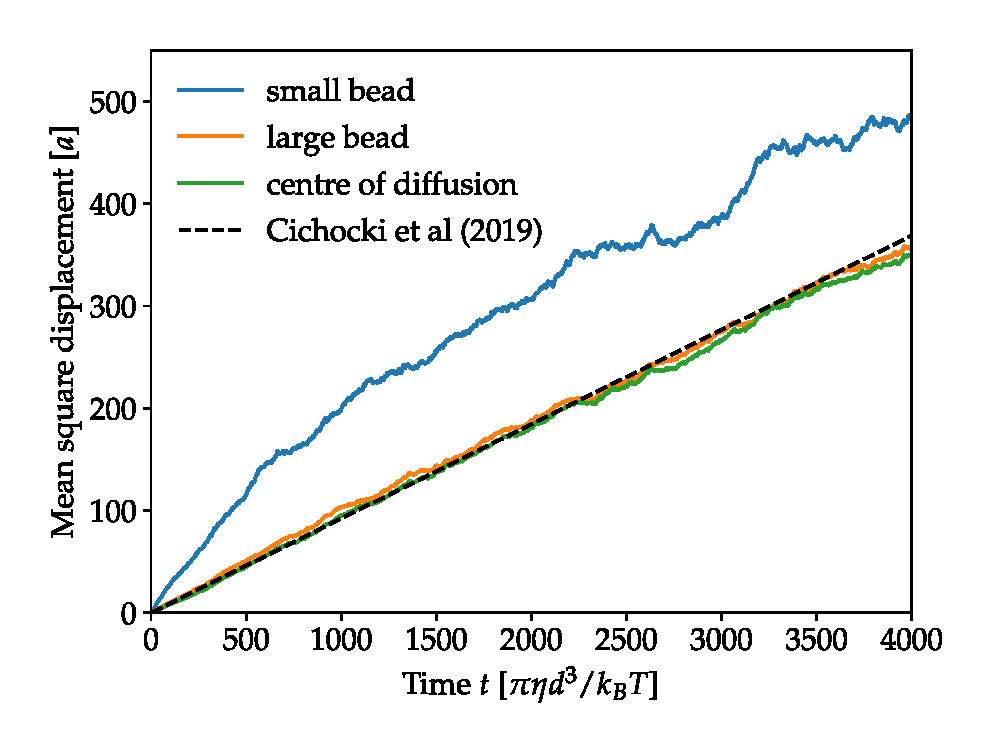
\includegraphics[height=0.3\linewidth,valign=t]{figures/mean_square_displacement.eps}
    \end{tabular}

    \caption{a) Representative configurations of an elastic molecule taken from a Brownian Dynamics simulation.
        b) Mean square displacement of three different tracked locations: the small bead at the end of the chain (blue), the large bead at the other end (orange) and the weighted average of all four beads compared with similar simulation from \textcite{Cichocki_2019} (dashed line).
        After a long enough time the slope of the mean square displacement is the same regardless of the point tracked.
        Graphics CC BY 4.0\cite{Waszkiewicz_2023_pychastic} } \label{fig:dl_and_ds}
\end{figure}

An intuitive first guess is to track 'the middle' or geometric average of molecules constituent parts, whereas slightly more refined approach is to use centre of mass -- this is clearly not an optimal strategy as shown by the exact result for the rigid molecule.
Location, or more specifically, the weights in the weighted average, have to be derived from the hydrodynamic properties rather than from, hydrodynamically irrelevant, mass.

Treating translational mobility $\mm{\mu}^{tt}$ as a tensor (with indices space, space, bead, bead) we can definite an inverse matrix of per-particle ensemble-average traces of mobility $b$ as
\begin{equation}
    \mm{b}_{ij} \left(\left< \mm{\mu}^{tt} \right> \right)_{jkll} = \mm{\delta}_{ik}
\end{equation}
where $\left< \cdot \right>$ denotes ensemble average.

Then the hydrodynamic radius is estimated by
\begin{equation}
    R_h \approx \frac{1}{2 \pi \eta} \left( \sum_i \sum_j \mm{b}_{ij} \right)^{-1}.
\end{equation}
We called this approach the minimum dissipation approximation (MDA) as explained in \textcite{Waszkiewicz_2024_mda}.
A complete derivation of the MDA method can be found in \textcite{Cichocki_2019}.

Clearly the MDA method (and earlier, simpler Kirkwood-Reismann method \cite{Kirkwood_1948}) require estimating ensemble averaged translational-grand-mobility matrix.
Given approximations \eqref{eqn:rotne-prager-translation}, we require only the relative positions of the constituent elements of the molecule and their effective sizes.
These should be drawn from the equilibrium distribution given by the Boltzmannian
\begin{equation}
    \dd p \propto \exp \left(- \frac{U}{k_B T} \right) \dd V.
\end{equation}
There are two potential difficulties with computing this measure: determining the potential energy $U$ and determining the volume element $dV$.
We discuss both of them in greater detail in \textcite{Waszkiewicz_2024_trimer}.
Both of these problems are more pronounced when very stiff springs are used as models of bonds leading to superficially paradoxical results such as the 'trimer paradox' discussed therein.

The methods discussed above have broad applicability, but now we turn our attention to specific examples of molecules studied in this thesis to highlight their distinct physical properties.
The stiffness of various molecules varies significantly, spanning many orders of magnitude, which in turn motivates the use of different modeling approaches in different cases.
We will outline the methodology leading to these diverse approaches in the following sections.

\section{Elastic macromolecules}

Soft matter as a discipline of physics evolved out of 'colloid suspensions science' under the influence of two 'fuel sources' -- bio-relevant measurements showing immediate applicability and a chase of observations of 'universal' validity, with universal being interpreted as insensitive to bio-chemical details of the molecules.
A good example of intersection of these two currents are models of long polymeric chains -- first elastic macromolecules to be successfully modelled.
These include some synthetic plastics but also bio-molecules such as DNA or denatured proteins.
A celebrated result of Rouse $R_h \sim N^{1/2}$ for a Gaussian chain with $N$ elements \cite{Rouse_1953} later improved by Zimm by inclusion of excluded volume interactions \cite{Zimm_1956} $R_h \sim N^\gamma$ with $\gamma=0.588$.
For a more detailed overview the subject matter see \textcite[chapter 3]{Dhont_2008}.
These scalings are valid under the assumption of small persistence length $P = EI / (k_B T)$, which captures the ratio of elastic forces (proportional to rigidity $EI$) to Brownian forces (proportional to fluctuation energy $k_B T$).

In reality there are more forces influcencing the conformation of macromolecules, their relative importance is easiest to compare using lengthscale ratios, which quantify the respective ranges of different interactions within the molecule.
In our case, the lengthscales of interest include the already mentioned persistence length, the building block size (quantifying excluded volume interactions), and the Debye length (quantifying electrostatic interactions, scaling with the inverse square root of the ionic strength $C_s$ of the buffer).
Some values of these lengthscales, pertinent to the publications \cite{Waszkiewicz_2023_dna} and \cite{Waszkiewicz_2024_mda}, are outlined in Table~\ref{tab:lengthscales}.
The need for assessing relative values for each problem is apparent -- there is a factor $160$ difference in stiffness of protein linkers and DNA filaments.

\begin{table}[htbp]
    \centering
    \begin{tabular}{llrr}
        \toprule
        \textbf{Description} &
        \textbf{Scaling}     &
        \textbf{IDP [\AA]}   &
        \textbf{DNA [\AA]}                                              \\
        \midrule
        Length               & $L$                     & 2000 & 1000    \\
        Persistence length   & $P = EI / k_B T$        & 3    & 500     \\
        Building block       &                         & 4    & 3       \\
        Debye length         & $R_D \sim (C_s)^{-1/2}$ & 1    & 1       \\
        \midrule
        Applicable limit     &                         & hot  & cold(?) \\
        \bottomrule
    \end{tabular}
    \caption{Relevant length scales for the two studied problems.
        Length row represents typical values.
        Debye length computed for relevant (physiological) buffer conditions.
    } \label{tab:lengthscales}
\end{table}

The first type of molecules investigated in this doctoral thesis are DNA minicircles, whose persistence length is comparable to the length of the very short DNA minicircles under investigation by the group of Professor Lynn Zechiedrich at Baylor College of Medicine.
Consequently, their conformation is primarily determined by the minimization of elastic forces and is relatively stable.

The second type of molecule investigated in this thesis is intrinsically disordered proteins (IDPs).
Their persistence length is two orders of magnitude smaller and comparable to the building block size (the $C_\alpha$ distance between consecutive amino acids along the chain).
This characteristic leads to a large conformational variability in an equilibrium ensemble, making both measurement and modeling challenging.

Much of the theoretical enthusiasm in developing complex models of IDPs, with a multitude of interactions, is hampered by an insufficient quantity or quality of experimental calibration data necessary for the determination of molecular "material constants".
In polymer science domains where data is plentiful, such as the area of globular proteins that can be readily measured by techniques like X-ray crystallography, significant numerical progress has been made using machine learning techniques, leading to celebrated examples like AlphaFold \cite{Jumper_2021}, which has achieved even popular science recognizability.

Progress in the domain of IDPs is much more modest, even though they constitute a large proportion of proteins \cite{Ward_2004} and play an important role in multiple bio-relevant processes, such as the functioning of the COVID-19 virus \cite{Rozycki_2022} (to name just one example particularly resonant in 2024).
In the opinion of the author this progress is (at least in part) determined by the amount of readily available experimental data -- compare over 200 thousand conformations available in the Protein Data Bank \cite{rcsb_org} with not even 50 high quality measurements of the diffusion coefficients of the IDPs we were able to extract from published works \cite{Waszkiewicz_2024_mda} or 118 proteins in the Small Angle Scattering Database \cite{sasdb_org}, or 462 proteins in the Protein Ensemble Database \cite{proteinensemble_org}.

Simultaneously, a variety of biochemical insights into both folded and disordered protein behavior invite phenomenological models with many covariates to explain the hydrodynamic size of these molecules.
A specific example of such insight could be the relative rigidity of polyhistidine fragments and tags.
Their presence (or, more simply, the share of histidines in the totality of amino acids forming a molecule) is sometimes used as an explanatory variable in the process of phenomenological modeling \cite{Tomasso_2016, Marsh_2010}.

As data concerning the hydrodynamic properties of IDPs is scarce, and a direct intervention in the protein sequence can be prohibitively expensive, since the synthesis of each new protein construct can take months, we encounter an issue more familiar to social scientists than physicists.
The available information essentially forms an observational study where correlation is difficult to separate from causation\footnote{This is in contrast to a typical physics experiment, akin to a randomized controlled trial in a social setting, where the experimenter is free to choose the value of the control variable and measure the outcome.
    In the example study of his-tag influence, we cannot simply randomly separate proteins into two groups and add or remove his-tags as required.
}.
Even if we perform all statistical analyses correctly and observe a statistically significant correlation between, for example, the presence of a his-tag and an increase in hydrodynamic size, how can we be sure that it is not simply a case of a confounding cause?
One can easily imagine a scenario where compact proteins containing a his-tag are simply harder to synthesize, leading to a distorted sample (selection bias) and forming our phenomenological conclusion based on biased data.
Correlations estimated this way can even have the opposite sign to the real causal effect, which is what we are really trying to estimate.
A comprehensive and approachable overview of the discrepancies between causal and correlational findings in observational studies can be found in \textcite{Cinelli_2022}.
For a more introductory exposition, refer to \textcite{Neal_2020}.

Until and unless we have a very large dataset of hydrodynamic properties of a bias-free, representative subset of IDPs, first principles theoretical models should take precedence over phenomenological models.
This is not just because of their precision, as demonstrated in \textcite{Waszkiewicz_2024_mda}, but also because they correctly model the causal dependency between the covariates of interest and hydrodynamic size.

\section{Diffusion coefficients in hot and cold limits}

First principles models of elastic molecules come in two flavors: atomistic and coarse-grained.

Atomistic methods, as outlined by \textcite{Karplus_1990}, can be utilized, albeit with certain challenges.
These methods either involve the explicit simulation of surrounding water molecules, demanding significant computational resources, or employ an implicit solvent scheme, both of which pose notable numerical difficulties \cite{Frenkel_2001}.
Even if simulations are theoretically feasible, generating 10-100 millisecond long trajectories for the direct computation of long-time diffusion coefficients, using this method requires great computational power.

On the other hand, coarse-grained methods utilize larger units, typically amino acid residues for proteins, as building blocks for conformation prediction schemes.
These units are integrated with a separate hydrodynamic model to predict diffusion coefficients.

Addressing the problem directly, even within a coarse-grained perspective, still presents numerical challenges.
Furthermore, the identification of a minimal model capable of reproducing experimentally observed variations in diffusion coefficients holds intrinsic value, offering a direct interpretation of observed variability through a restricted set of molecular mechanisms.
In this context, two different minimal models, termed the ``cold limit'' and ``hot limit,'' (inspired by the naming conventions such as \cite{Murphy_2018,Bleibel_2014}) were employed to simulate the conformations of two classes of molecules: DNA minicircles and Intrinsically Disordered Proteins (IDPs).

A comparison of persistence length to the minicircle length and a visual examination of CryoEM figures from \textcite{Irobalieva_2015} alongside equilibrium configurations of twisted beams as described by \textcite{Coleman_2000} suggested that thermal fluctuations might exert only a minor influence on the overall behavior of these molecules.
Consequently, the problem was modeled in the ``cold limit'' (cf.
Table~\ref{tab:tickmarks}), where thermal fluctuations were neglected, and only equilibrium configurations were computed, akin to operating at negligible absolute temperature.
Subsequently, these configurations were treated as rigid bodies when determining the hydrodynamic radius, as detailed in \textcite{Waszkiewicz_2023_dna}.
The influence of thermal fluctuations was further investigated using the \code{pychastic} package post-publication.

The second type of molecule investigated in this study was the intrinsically disordered proteins (IDPs).
These molecules exhibit much smaller stiffness, with a persistence length as small as $3$ \AA{} and an elastohydrodynamic length scale ($8\pi^3 EI / (L^2 g \rho)$) of approximately $2000$ \AA{} -- comparable to the molecule's length.
This characteristic further justifies our initial concern regarding the potential influence of buckling forces arising in sedimentation on hydrodynamic sizes in AUC measurements.
Fortunately, the group led by Prof.
Anna Niedzwiecka at the Institute of Physics, Polish Academy of Sciences, employs fluorescence correlation spectroscopy (FCS) instead of AUC, which does not introduce large force gradients on the molecule.
Given that the persistence length is comparable to the building block size, we decided to focus on the \emph{hot limit} of the problem, where elastic forces are disregarded relative to thermal fluctuations (however, the excluded volume interactions do not vanish at high temperatures; thus, this approach can be treated as a $\lim T \to \infty$ approximation, hence the name).
More precisely, bending forces arising from the Ramachandran angles distributions were neglected, while the forces governing bond length were taken to be infinitely strong.
This approach requires care when handling bond-angle distributions, and some apparently paradoxical results can arise, as discussed in \textcite{Waszkiewicz_2024_trimer}.
We show that the intuitive distribution 'uniform on a sphere' indeed arises as a limit in the case of linear filaments (notably, a different distribution arises for molecules with loops as shown therein, with deviations in probability density that can be arbitrarily large).

\begin{table}[htbp]
    \centering
    \begin{tabular}{llll}
        \toprule
        \textbf{Manuscript}                                        &
        \textbf{Elasticity}                                        &
        \textbf{Thermodynamics}                                    &
        \textbf{Hydrodynamics}                                                                            \\
        \midrule
        DNA \cite{Waszkiewicz_2023_dna,Waszkiewicz_2021_stability} & \checkmark & .          & \checkmark \\
        IDP \cite{Waszkiewicz_2024_mda,Waszkiewicz_2024_trimer}    & .          & \checkmark & \checkmark \\
        Pychastic \cite{Waszkiewicz_2023_pychastic}                & \checkmark & \checkmark & \checkmark \\
        \bottomrule
    \end{tabular}
    \caption{Three domains of interest for the study of elastic molecules.
        Very high and very low stiffness of DNA and IDPs respectively allowed us to use simplified models.
    }
    \label{tab:tickmarks}
\end{table}

The two experimentally inspired problems, even though solvable to a satisfactory degree within the presented approximations, leave a desire to assess the size of the error introduced by these particular simplifications.
These error estimates can be compared either to the precision of the experimental data or to the estimates of other approximation errors in the model, such as approximations of the hydrodynamic mobility tensors.
This can guide the effort in further improvements to the numerical method; for example, should we first work on including thermal fluctuations to the conformations or rather improve hydrodynamic mobility tensor approximations?

When mobility tensors are simply modeled with the Rotne-Prager approximation (such as the tensors of the \code{pygrpy} package), the errors introduced there are of the order of 2\% 

Assessing errors introduced by approximate conformer generation, whether in the hot ($T\to\infty$) or cold ($T\to0$) limit, necessitates simulating the ensemble at finite temperatures.
% (based on R8 test case of \cite{Zuk_2018}).
Various methods can be employed for this purpose, but a simulation grounded in physical principles holds particular appeal.
To achieve good performance, the Brownian Dynamics method was selected.
This approach relies on formulating the dynamical equation governing conformational changes in the form of an SDE.

Surprisingly, in 2022, the authors found that the only high-quality SDE integration package available was \code{differentialequations.jl} in Julia \cite{Rackauckas_2017}.
Since Julia is still not very popular among physicists (or at least not inside the soft-matter community), this resulted in frequent re-implementation of SDE integration methods for each problem and often re-implementation of the hydrodynamic interaction tensors as well (possibly due to the fact that the Rotne-Prager-Yamakawa tensors most frequently used in our group were originally implemented in Fortran \cite{Zuk_2018}).

We have tried to address this issue by ensuring that the packages \code{pychastic} (for SDE integration) and \code{pygrpy} (for Rotne-Prager-Yamakawa tensors) are easily accessible -- with single command installation and compatibility across various operating systems including Linux distributions, MacOS, and (as of 2023) even Windows 10 \cite{jax_on_windows}.
Additionally, substantial effort has been invested in creating straightforward yet realistic examples in the documentation.
This not only simplifies the learning curve but also aims to encourage wider adoption of our integration package.
For a comprehensive understanding of implementation and usage, please refer to the detailed information provided in \textcite{Waszkiewicz_2023_pychastic}.

The specific implementation of \code{pychastic} further streamlines the development of similar models by eliminating the need for explicit force specification.
Instead, users can now simply define the energy, and the forces can be derived programmatically using \code{jax.grad} without compromising speed and precision.
This feature proved particularly advantageous in simulating shear-relaxed dynamics of DNA minicircles, where the energy depends on the non-local quantity of writhe ($Wr$).

The answer to the correct development direction (in the opinion of the author) lies in future experimental data with resolutions capable of probing inaccuracies of the force-fields used or showing clear dependencies on buffer conditions such as temperature or ionic strength.
Such measurements are in progress, and early results provide insights into future DNA models \cite{Ranasinghe_2023}.

\section{Experimental techniques}

For the author, the experimental challenges of studying biomacromolecules have been an eye-opening lesson in patience.
The excellent work on biosynthesis by the groups at Baylor College of Medicine and the Institute of Physics of the Polish Academy of Science should not be underestimated.
These two collaborations provide an overview of many experimental challenges: from the success or failure of initial biosynthesis, obtaining correct concentrations, to purification from by-products of biosynthesis and the stability of the resultant molecular constructs, to practical obstacles such as replacing discontinued lab equipment and cross-border shipping.

Even if everything aligns and one obtains a good sample of the molecule to study, the measurement itself is no easy task either.
Both AUC and FCS methods rely on time-series analysis of an optical signal -- in that sense, they are both indirect methods requiring model fitting within the experimental procedure.
This complicates the analysis of direct measurement error (uncertainty of a single measurement), with the current Monte Carlo-based AUC analysis method providing no uncertainty estimates for samples of high purity.
However, single measurement error is not the only, and not even the leading, source of uncertainty in the measurements of the diffusion (and sedimentation) properties of the molecules.
Since buffer conditions, concentration, and even the time from synthesis \cite{Nag_2011} affect the final outcome, these factors must be incorporated into error analysis to arrive at a comprehensive confidence interval for the measurements.
Unfortunately, some authors do not provide any error estimates \cite{Poznar_2017, Khaymina_2007}, and most of them do not discuss multiple sources of error.

The following sections describe the theoretical underpinnings of the experimental methods relevant to the publications included in this thesis.

\subsection{Analytical Ultracentrifugation}
\label{sec:AUC}

\begin{figure}[h]
    \centering
    \begin{tabular}{llll}
        a)                                                                                      &
        \includegraphics[height=0.3\linewidth,valign=t]{figures/ultracentrifugation_device.png} &
        b)                                                                                      &
        \includegraphics[height=0.3\linewidth,valign=t]{figures/ultracentrifugation_results.png}
    \end{tabular}

    \caption{a) Rotor from an ultracentrifuge. b) Haemoglobin concentration profiles from an early AUC experiments with rotor spinning at 42'000rpm or 104'000 G.
        Profiles derived from photographs taken at 30 minute intervals are compared with Lamm equation predictions (dashed).
        Reprinted with permission from \cite{Svedberg_1927}.
        Copyright 1927 American Chemical Society.
    }
    \label{fig:auc_diagram}
\end{figure}

Analytical Ultracentrifugation (AUC) is one of the oldest techniques in the domain of colloidal science receiving a Nobel prize in 1926.
In AUC a colloidal suspension is put inside a rapidly rotating centrifuge to increase the sedimentation rate of the molecules (current centrifuges spin with G-forces as large as 10'000G).
Inside the centrifuge rotor a small window allows for optical measurements of either absorption or transmission (in recent models involving multiple wavelengths) which change as a result of concentration variation.

Changes of concentration inside the container are governed by the Lamm equation containing the divergence of two currents: diffusive -- proportional to concentration gradient and sedimentation -- proportional to local outward acceleraiton
\begin{equation}
    \frac{\pd \phi}{\pd c} = \nabla \cdot \left( D \nabla \phi + s \omega^2 \bm{R} \phi \right).
    \label{eqn:lamm-equation}
\end{equation}

Derivation of the $s$ and $D$ values from experimental, time-dependent concentration profiles is done via a fitting procedure which requires efficient solution schemes for the PDE~\eqref{eqn:lamm-equation}\cite{Demeler_2016,Cao_2005}.
The finite element method combined with nonlinear least-squares techniques and Monte-Carlo based error estimation gives both values and uncertainties of the $s$ and $D$ values which can be used to determine other molecular parameters such as $R_h$ or molecular mass.

\subsection{Fluorescence Correlation Spectroscopy}
\label{sec:FCS}

The overview of the Fluorescence Correlation Spectroscopy (FCS) technique follows that of \textcite{Tompson_2002} and \textcite{Gregor_2008}.
The FCS method, introduced about 50 years after invention of AUC, relies on temporal analysis of fluorescence signal to determine properties of the studied sample.
These include the hydrodynamic size (relevant to this work), but it is also possible to determine adsorption or reaction kinetics using this method.

In the case of diffusion constant measurements, a very dilute sample of studied molecule (typically marked with an added fluorophore) is illuminated by a laser inside a confocal microscope.
Excited fluorophore then emits light back through the microscope but at a slightly shorter wavelength (due to the Stokes shift) which reaches the detector shielded from laser light with a dichroic mirror (cf Fig.~\ref{fig:fcs_diagram}).

Recorded fluorescence signal $F(t)$ is time dependent, since the number of molecules inside the laser beam changes in time due to diffusion.
FCS experiments perform best when at each moment expected number of excited molecules is close to one giving largest relative fluctuations of the fluorescence signal.

\begin{figure}[h]
    \centering
    \begin{tabular}{llll}
        a)                                                                           &
        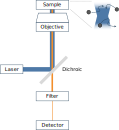
\includegraphics[height=0.4\linewidth,valign=t]{figures/fcs_setup_clean.pdf} &
        b)                                                                           &
        \includegraphics[height=0.4\linewidth,valign=t,trim=0 0 0 0.5cm]{figures/fcs_data_and_fit.pdf}
    \end{tabular}

    \caption{a) A typical FCS setup diagram  b) Fluorescence correlation spectroscopy (FCS) data with a fited a model for 3d diffusion (\textcite{Waszkiewicz_2024_mda}
        CC-BY-NC 4.0)} \label{fig:fcs_diagram}
\end{figure}

The frequency of the fluctuations due to diffusion can be quantified (and thus used to derive the diffusion coefficient) by considering signal autocorrelation function $G(\tau)$ given by 

\begin{equation}
    G(\tau) = \left< F(t) F(t-\tau) \right>
\end{equation}
with $\left< \cdot \right>$ denoting time average.
This function is composed of two terms -- constant background (in the case of non-interacting molecules) term due to photons coming from two different molecules and a delay dependent term quantifying probability of detecting a photon from the same molecule again.
For simplicity of this overview, we focus only on the last term.

Suppose for simplicity that a position-dependent probability of excitation describing the shape of the excitation volume can be described by a axisymmetric Gaussian profile $U(\bm{r})$ given by
\begin{equation}
    U(\bm{r}) = \kappa \exp\left( - \frac{2}{a^2} \left( x^2 + y^2 \right) - \frac{2}{b^2} z^2 \right), \label{eqn:excitation_profile}
\end{equation}
with $\bm{r} = [x,y,z]$ and $\kappa$ is some overall constant.

If we now consider the Green's function $g(\bm{\rho},\tau)$ of the diffusion problem given by 

\begin{equation}
    g(\bm{\rho},\tau) = \frac{1}{(4\pi D \tau)^{3/2}} \exp\left( - \frac{|\rho|^2}{4 D \tau}\right)
\end{equation}

we can express the autocorrelation function according to 

\begin{eqnarray}
    G(\tau) & = & \int \int U(\bm{r} + \bm{\rho}) g(\bm{\rho},\tau) U(\bm{r}) \dd \bm{r} \dd \rho \\
            & = & \frac{\pi^{3/2}}{8} \frac{a^2 b}{(1+4 D \tau / a^2)\sqrt{1+4D\tau/b^2}}.
    \label{eqn:fcs_theory}
\end{eqnarray}

Since the parameters $a$ and $b$ cannot be known a priori, one typically fits a simplified expression 

\begin{equation}
    G(\tau) = G(0) \left( \left(1+\frac{\tau}{\tau_D}\right) \left(1 + \gamma \frac{\tau}{\tau_D}\right)^{1/2} \right)^{-1} + G(\infty), \label{eqn:fcs-autocorrelation}
\end{equation}
where $\gamma$ quantifies the aspect ratio of the excitation volume and $\tau_D$ characteristic time of the diffusion.
We can obtain diffusion coefficient $D$ from the residence time by comparing a reference sample of known $D$ and computing a ratio.

\subsection{Small Angle X-ray Scattering}
\label{sec:SAXS}

This section follows notation of \textcite{Hermann_2008}.
Another experimental technique is based on the analysis of the X-ray scattering on the colloidal particles as a function of the beams deflection vector $\bm{q}$ defined as a difference between incoming wave vector $\bm{k}_i$ and scattered wave vector $\bm{k}_s$.

\begin{figure}[h]
    \centering
    \includegraphics[width=0.6\linewidth]{figures/scattering_diagram.pdf}
    \caption{Phase shifts in Born approximation.}
    \label{fig:saxs_diagram}
\end{figure}

For colloidal particles, the Born approximation of single-event scattering (as show in fig.~\ref{fig:saxs_diagram}) is a sufficient description to model experimental data.
Within this approximation, the scattering pattern is computed as an interference pattern of the scattered signals from different scattering sites due to phase shift $\Delta \Phi$ resulting from difference in optical path length.

\begin{equation}
    \Delta \Phi = \bm{R}_{ij} \cdot (\bm{k}_s - \bm{k}_i) = \bm{R}_{ij} \cdot \bm{q}
    \label{eqn:scattering-phase-shift}
\end{equation}

We can express the complex amplitude of the scattered wave $A(\bm{q})$ as a Fourier transform of the scattering intensity distribution $\rho(\bm{r})$.

\begin{equation}
    A(q) = A_0 \int \rho(\bm{r}) \exp(i \bm{q} \cdot \bm{r}) \dd \bm{r} \label{eqn:scattering-amplitude-integral}
\end{equation}

Since the observed intensity on the screen $I$ is proportional to the squared absolute value of the wave amplitude $I(\bm{q}) \propto |A(\bm{q})|^2$, we can express $I(\bm{q})$ as a double integral 

\begin{eqnarray}
    |A(\bm{q})|^2 & = & A A^{*}                                                                                                            \\
                  & = & A_0^2 \int \int \rho^{*}(\bm{r}') \rho(\bm{r}'') \exp(i \bm{q} \cdot (\bm{r}'-\bm{r}'')) \dd \bm{r}' \dd \bm{r}''.
    \label{eqn:intensity-profile-integral}
\end{eqnarray}

If we assume that the scattering sites are point-like, we can express the scattering density distribution as a sum of Dirac distributions $\delta$ centred at locations of scattering sites $\bm{s}_i$ 

\begin{equation}
    \rho(\bm{r}) = \sum_i \rho_i \delta(\bm{r}-\bm{s}_i),
\end{equation}
where $\rho_i$ gives scattering intensity on site $i$.
The integral \eqref{eqn:intensity-profile-integral} reduces to a double sum 

\begin{equation}
    I(\bm{q}) = A_0^2 \sum_i \sum_j \rho_i \rho_j \exp(i \bm{q} \cdot (\bm{s}_i - \bm{s}_j)).
\end{equation}

Inside the colloid, the distribution of orientations of the macromolecules with respect to the lab frame is invariant under action of rotations.
For a vector $\bm{v} = \bm{s}_i - \bm{s}_j$ this simply implies $\bm{v}$ distributed uniformly on a sphere and its projection onto a vector $\bm{q}$ distributed uniformly on an interval according to orange slicing theorem\footnote{the orange slicing theorem: if you slice an orange into slices of equal thickness each slice has the same share of the orange peel} giving 

\begin{eqnarray}
    \left< I(\bm{q}) \right> & = & A_0 \sum_i \sum_j \rho_i \rho_j \int \exp(i q s) \mathbb{I}(|s| < |\bm{s}_i - \bm{s}_j|) \dd s \\
                             & = & A_0 \sum_i \sum_j \rho_i \rho_j \operatorname{sinc}(|q||\bm{s}_i - \bm{s}_j|)                  \\
                             & = & A_0 \sum_i \sum_j \rho_i \rho_j \operatorname{sinc}(|q||\bm{R}_{ij}|).
\end{eqnarray}

Thus, the prediction of the scattering intensity of in a SAXS measurement of a colloidal suspension reduces to the computation of the distance matrix $R_{ij}$ between scattering sites, given the values of scattering intensities $\rho_i(q)$.
In the case of elastic macromolecules, the scattering signal is simply averaged over an ensemble of possible molecular conformations.
With the help of tabulated values of scattering intensities of each amino-acid obtained by \textcite{Tong_2016}, a python package \code{saxs_single_bead} was developed.

\chapter{Software packages}

Most of the source code utilized in the preparation of this thesis has been made available in public repositories on GitHub.
Furthermore, in the instances detailed below, considerable effort was invested in structuring the software into Python packages with structured documentation to facilitate ease of use.

\begin{table}[htbp]
    \centering
    \begin{tabular}{llll}
        \toprule
        \textbf{Package}         &
        \textbf{Description}     &
        \textbf{GitHub}          &
        \textbf{Docs}                                                                                                             \\
        \midrule
        \code{pychastic}         & SDE solver                          & \cite{gh_pychastic}         & \cite{rd_pychastic}        \\
        \code{pygrpy}            & Rotne-Prager mobility tensors       & \cite{gh_pygrpy}            & \cite{rd_pygrpy}           \\
        \code{glm_mda_diffusion} & GLM+MDA diffusion calculator        & \cite{gh_glm_mda_diffusion} &                            \\
        \code{sarw-spheres}      & Globule-linker conformer generator  & \cite{gh_sarw_spheres}      &                            \\
        \code{saxs-single-bead}  & One site per amino-acid SAXS engine & \cite{gh_saxs_single_bead}  & \cite{rd_saxs_single_bead} \\
        \code{pywrithe}          & Computing writhe of a curve         & \cite{gh_pywrithe}          & \cite{rd_pywrithe}         \\
        \bottomrule
    \end{tabular}
    \caption{Software packages developed in the course of preparation of this doctoral thesis.}
    \label{tab:packages}
\end{table}

\chapter{Main results of the thesis}
\clearpage

\begin{publicationpage}{Waszkiewicz_2021_hydrodynamic}{Hydrodynamic effects in the capture of rod-like molecules by a nanopore}
    \commentary{
        %1. Topic relevance

        Translocation of biomolecules through nanopores lies at the heart of many biological processes, such as cell signalling.
        It is a significant element of modern nanotechnology and sequencing techniques which give access to the structure of DNA or RNA in small quantities.
        Thus, it enables low-cost genotyping and testing without the need to resort to PCR amplification or chemical labelling.
        In a relevant experimental setup for DNA analysis, the efficiency of sequencing hinges on two critical factors: the translation speed through the nanopore and the capture radius of the nanopore.

        %2. Literature overview
        The complex process of translocation is now understood in great detail and has been studied extensively to assess the importance of multiple contributing factors.
        However, the process of approach and capture by a nanopore still poses a challenge.
        Existing models of capture mostly overlook hydrodynamic interactions which might play an important role when the DNA fragment is sufficiently close to the nanopore.
        This work aimed to fill this gap by discerning and examining the time scales associated with different modes of motion -- rotational and translational -- induced by different types of forces present in the system: Brownian fluctuations, electrostatic attraction to the pore, and hindering effects of hydrodynamic interaction with the wall.
        By the analysis of different regimes, we successfully identified the pore distance at which wall interaction terms exert a dominant influence and therefore should be accounted for in quantitative models.

        %3. What techique was used
        To perform the analysis, we constructed a simple coarse-grained model of an anisotropic, rod-shaped particle, representing the elongated nature of a DNA filament of length short compared to its persistence length.
        In such a case the molecules can be treated as a stiff rigid body, for which an approximate form of the mobility tensor in the presence of a wall has been proposed \cite{Lisicki_2016}.
        In this work, we performed scaling analysis to identify the regimes where different types of forces are dominant.
        %4. What was the outcome        
        We then calculated the trajectories of a model nanorod near a wall in Mathematica, incorporating the near-wall corrected mobility tensor, which takes into account both the anisotropy of the particle itself, and its coupling to the wall.

        %5. PhD candidate
        In this study, the PhD candidate: co-developed the scaling analysis and the theoretical description, implemented the near-wall corrections to the mobility tensors and generated all numerical results and visualisations presented, participated in the analysis of results, prepared all figures, wrote the first draft and edited all subsequent versions.
    }

\end{publicationpage}
\includepdf[pages={-}]{publications/waszkiewicz_2021_hydrodynamic}

\begin{publicationpage}{Waszkiewicz_2021_stability}{Stability of sedimenting flexible loops}
    \commentary{
        %1. Topic relevance   
        Analytical Ultracentrifugation, a method for determination of hydrodynamic radius and effective density of a molecule, involves applying extremely high centrifugal forces to a colloidal suspension.
        This well established technique has been successfully used to measure various colloidal particles, however, its application to flexible macromolecules raises concerns over the influence of large forces (or more precisely large force gradients) imposed on the molecule.
        In extreme cases high values of compression in the fore of the sedimenting particle can lead to buckling in sedimentation processes.
        To understand when this might happen, we focused on an idealised problem involving the sedimentation of a circular fibre, aiming to eliminate end-corrections from the buckling consideration.

        %2. Literature overview
        Earlier studies of sedimenting flexible rings using bead-model approach \cite{Gruziel_2018} showed complex dynamics with a wide variety of periodic orbits depending on setup parameters and initial conditions.
        Assessing which parts of this complexity are attributable to hydrodynamic interaction, which to bead-model discretisation and which are intrisic to similar setups was a secondary goal of this investigation.

        %3. What techique was used
        To determine the cases where buckling may occur we performed linear stability analysis within the Resistive Force Theory approximation under which hydrodynamic drag is a local quantity.
        Under this simplification the tension inside the loop at each moment can be computed from an ordinary differential equation.

        %4. What was the outcome        
        We calculated the evolution of the conformation of a sedimenting loop using a custom numerical integrator based on a truncated Fourier series.
        These results were compared with a linear stability analysis of the initial, circular configuration, which provides a near analytical stability boundary.
        We obtained good agreement between numerical and analytical approaches and favourable comparison with earlier work.

        %5. PhD candidate
        In this study, the PhD candidate: co-developed the theoretical description, conducted a stability analysis of the PDE and computed the stability criterion using the proposed matrix method, generated all numerical results and visualisations presented, prepared all figures, wrote the first draft and edited all subsequent versions.
        Additionally they are a corresponding author.
    }
\end{publicationpage}
\includepdf[pages={-}]{publications/waszkiewicz_2021_stability}

\begin{publicationpage}{Waszkiewicz_2023_dna}{DNA supercoiling-induced shapes alter minicircle hydrodynamic properties}
    \commentary{
        %1. Topic relevance

        Bio-relevance of the DNA requires little introduction.
        Even though the basic structure of the DNA is well understood at least since the 1950s, understanding the secondary structure of the DNA filament remains an an important but challenging task.
        Since the overall 3D conformation of the DNA can influence gene expression, understanding the forces governing its elasticity is crucial.
        By using a selection of small DNA loops which differ only in the linking number, we were able to measure conformational changes of the DNA via its hydrodynamic properties in the diffusive measurements.

        %2. Literature overview
        Earlier works such as \textcite{Coleman_2000} established the correct energy density functional for modelling slender loops subject to torsional stress.
        Unfortunately the original code giving piecewise analytical solutions for the problem is lost and thus re-implementation of the solver was required.
        That work used DNA loops as inspiration but was never directly tested against experimental results.
        On the other hand a variety of software packages are capable of predicting hydrodynamic radius given shape of a rigid molecule (Zeno, US-Somo, GRPY), but as far as we know, they were not yet used for prediction of hydrodynamic properties of DNA loops.

        %3. What techique was used
        This study emerged from the collaborative efforts of three distinct groups.
        The first group, specialising in theoretical modelling, comprised the PhD candidate, Maciej Lisicki, and Piotr Szymczak from the Faculty of Physics, Univeristy of Warsaw and Maria L Ekiel-Jeżewska from the Institute of Fundamental Technological Research, Polish Academy of Sciences.
        The second group, responsible for the biosynthesis of DNA minicircles, included Jonathan M Fogg, Daniel J Catanese Jr, and Lynn Zechiedrich from the Department of Pharmacology and Chemical Biology at Baylor College of Medicine and Rice Univeristy.
        The third group, overseeing AUC measurements, included Maduni Ranasinghe and Borries Demeler from the Department of Chemistry and Biochemistry at the University of Lethbridge.

        The choice of topoisomers of DNA minicircles as the subject of collaboration proved strategic.
        For the modelling group, the shared hydration properties among different topoisomers and their loop structure, as opposed to rods, facilitated a more straightforward modelling process.
        The biosynthesis group leveraged their prior experience in preparing these molecules, coupled with an interest in understanding the physical origins of changes in the bio-activity of writhed DNA.
        Lastly, for the AUC group, the remarkable sample stability of DNA minicircles allowed for numerous re-runs of experiments.

        %4. What was the outcome
        Using the selected approach, we were able to calibrate the hydrodynamic thickness of the DNA filament against measurements of the configurations which adopt toroidal shape and use that value to predict the hydrodynamic radius of all topoisomers that were experimentally measured.

        %5. PhD candidate
        In this study, the PhD candidate: proposed and implemented a numerical method to obtain equilibrium configurations of the supercoiled DNA minicircles.
        They computed the hydrodynamic properties of these configurations using GRPY, pygrpy, and Zeno software (with only Zeno being included in the published manuscript); wrote the first draft and edited all subsequent versions of the manuscript, produced all graphs and visualisations incorporated in the manuscript.
    }
\end{publicationpage}
\includepdf[pages={-}]{publications/waszkiewicz_2023_dna}

\subsection{Comment: Thermal Effects on the Shapes of DNA Minicircles}

One model limitation of publication \cite{Waszkiewicz_2023_dna} was a limited assesment of the influence of thermal fluctuations on the shape and hydrodynamics of DNA loops.
This was caused by lack of readily available tools for Brownian dynamics simulation under nonlocal force fields -- such as the energy functional depending on writhe (which is a nonlocal quantity).

Utilising the later developed \code{pychastic} package, we conducted simulations to explore the shapes of DNA minicircles at finite (room) temperatures and computed their apparent diffusion coefficient using the minimum dissipation method described in \textcite{Cichocki_2019}.

In these simulations, we assumed that torsional stresses in the DNA are relaxed.
Consequently, the total elastic energy $E_{el}$ of such a minicircle is given by
\begin{equation}
    E_{el} = \frac{1}{2} \int_0^L EI \left( \kappa^2 + \omega \left( \frac{2\pi (Lk - Wr)}{L} \right)^2 \right) dl.
\end{equation}

Both $\kappa$ and $Wr$ can be computed from the shape of the centreline alone (or a suitable discretisation thereof), reducing the dimensionality of the problem compared to an approach where both the position and orientation of filament segments are simulated.
It is worth noting that simulating rotational dynamics, even of a single body, is a complex task, as outlined in \textcite{Waszkiewicz_2023_pychastic}.

Given that $Wr$ is a nonlocal quantity, the computation of forces from $E_{el}$ can be cumbersome.
Fortunately, this task can be accomplished with the assistance of \code{jax.grad}, which is compatible with the SDE solver \code{pychastic}.

This gives further insight into the intermediate region ($1 < Lk < 2.5$) where minicircles have multiple stable configurations at absolute zero temperature discussed in \textcite{Waszkiewicz_2023_dna}.

\begin{figure}[htbp]
    \centering
    \includegraphics[height=0.5\linewidth]{figures/with_thermal_effects.pdf}
    \caption{Hydrodynamic radius relative to $Lk = 0$ configuration of the 336bp minicircle as a function of the linking number.}
    \label{fig:thermalized_loops}
\end{figure}

It turns out that the effects of thermal fluctuations on the overall hydrodynamic radius outside of the intermediate region are negligible.
Moreover, the range of $Lk$ values for which the equilibrium ensemble contains both open configurations and configurations with self-contact is very small—less than 0.2 turns.
When considering the difference in total elastic energy between the flat circular configuration and the configuration with self-contact, one arrives at $\frac{\partial \Delta E}{\partial Lk} \approx Lk \frac{8\pi^2 \cdot}{3} \frac{P}{L} k_B T \approx 26 k_B T$, providing an estimate of the transitional region width of approximately $0.03$.
%TODO: redo this calculation and check
This contrasts starkly with CryoEM data \cite{Irobalieva_2015}, where a multitude of conformations were observed for a wide range of $Lk$ values.
One possible explanation for this discrepancy lies in the temperature dependence of the geometric properties of DNA, as hinted at by the results of \textcite{Ranasinghe_2023}.

The example above highlights our motivations for the development of the \code{pychastic} package which is described in detail in the next publication.
\clearpage

\begin{publicationpage}{Waszkiewicz_2023_pychastic}{Pychastic: Precise Brownian dynamics using Taylor-Ito integrators in Python}
    \commentary{
        %1. Topic relevance

        The major theoretical limitation in earlier studies revolved around the incomplete treatment of Brownian motion.
        Ref.~\cite{Waszkiewicz_2021_hydrodynamic}, dynamics was simplified to a 2D case due to Mathematica's inability to handle full $SO(3)$ dynamics, as outlined in the publication below.
        Similarly, in Ref.~\cite{Waszkiewicz_2023_dna}, the challenges arose from the nature of the Writhe quantity, leading to a non-local force field that made assessing the effects of thermal fluctuations on the shape of minicircles exceptionally challenging.

        %2. Literature overview
        Addressing the treatment of Brownian motion through stochastic differential equations presented a well-posed mathematical problem, with a range of solutions described for example in Ref.~\cite{Kloeden_1992}.
        However, surprisingly, there was no readily available, easy-to-use software solution, such as the package described in the publication below.

        %3. What techique was used
        We took advantage of the modern python features such as introspection and metaprgoraming which enable efficient automatic differentiaion of functions combined with the package \code{jax} for just-in-time compilation of python code to machine code for performance.

        %4. What was the outcome
        The resultant package, \code{pychastic}, is now available to instal via \code{pip} or directly from GitHub \cite{gh_pychastic}.

        %5. PhD candidate
        In this study the PhD candidate: conceptualized the problem, lead a small programming team, which included the author, Maciej Bartczak, and Kamil Kolasa, co-developed a Python package complete with documentation, examples, and tests, created test cases and debugging tools that facilitated the correction of multiple typos found in existing literature (outlined in the publication).
        Co-designed illustrative examples showcasing concrete applications of the tools developed during the thesis preparation.
        Additionally, he wrote the first draft and edited all subsequent versions of the manuscript.
    }
\end{publicationpage}
\includepdf[pages={-}]{publications/waszkiewicz_2023_pychastic}

\begin{publicationpage}{Waszkiewicz_2024_mda}{Minimum dissipation approximation: A fast algorithm for the prediction of diffusive properties of intrinsically disordered proteins}
    \commentary{
        %1. Topic relevance

        Intrinsically Disordered Proteins (IDPs) constitute a large class of bio-relevant elastic macromolecules.
        They typically consist of approximately rigid domains connected with flexible linkers.
        This type of molecule comprises up to a third of proteins in eukaryotes, yet remains understudied because it cannot be easily analysed using crystalographic techniques due to their ever changing confromations.
        Determining the relative imporance of diferent physical processes determining conformations of the IDPs and role of flexible linkers in interactions between their domains remains an open problem.

        %2. Literature overview
        To the best knowledge of the authors, this is the first publication comparing a first-principles approach (in contrast to many phenomenological attempts such as Ref.~\cite{Tomasso_2016,Forman-Kay_2022}) to prediction of hydrodynamic size of IDPs with experimental data.
        Earlier approaches to the prediction of the protein hydrodynamic radius (for example Ref.~\cite{Fleming_2018}) generally focus on techniques which approximate the protein as a rigid body.

        %3. What techique was used
        From a modelling perspective, intrinsically disordered proteins differ significantly from DNA.
        They consist of globular fragments connected with linkers, where the former are essentially rigid, and the latter are almost ideally flexible.
        Such proteins are ideal subjects for the application of the Minimum Dissipation Approximation, specifically designed for the fast computation of diffusion coefficients for molecules exhibiting substantial conformational variability and parts of varying sizes.

        This study emerged from the collaborative efforts of two distinct groups.
        The first group, specialising in theoretical modelling, included PhD candidate, Bogdan Cichocki, Maciej Lisicki and Piotr Szymczak from the Warsaw University Physics Department.

        The second group, responsible for synthesis and FCS measurements, comprised Agnieszka Michaś, Michał K.~Białobrzewski, Barbara P.~Klepka, Maja K.~Cieplak-Rotowska, Zuzanna Staszałek, and Anna Niedźwiecka from the Institute of Physics of the Polish Academy of Sciences.

        %4. What was the outcome
        We were able to obtain favourable comparison with experimental data, with substantially better agreeement than all phenomenological models selected for comparison and noticeably better agreement than simple power law fit.
        The resulting code was packaged into an easy to use python library and command line tool called \code{glm_mda_diffusion} ready to install via \code{pip} and available directly on GitHub.

        %5. PhD candidate
        In this study the PhD candidate: co-conceptualized the modelling approach, investigated the available conformer generation schemes, implemented the Python port \code{pygrpy} of the generalised Rotne-Prager mobility tensors (originally implemented in Fortran \cite{Zuk_2018}), implemented the globule-linker conformer generation scheme, performed numerical calculations and statistical analysis to assess deviations between theory and experiment.
        Additionally, they wrote the first draft and edited all subsequent versions of the manuscript.
    }
\end{publicationpage}
\includepdf[pages={-}]{publications/Waszkiewicz_2024_mda}

\subsection{Comparing Conformations to SAXS Data}
The author would like to thank dr.~Bartosz Różycki for his guidance regarding experimental SAXS data.

As detailed in \textcite{Waszkiewicz_2024_mda}, computing the diffusion coefficient for a given IDP requires generating samples from the equilibrium ensemble.
To assess the quality of the conformer generation method independently of hydrodynamic modelling, we utilised available SAXS data (which was not included in the final manuscript).
One example of such a comparison is illustrated in Figure~\ref{fig:saxs_compare}, where experimental data from \textcite{Sicorello_2021} is compared with our implementation of the globule-linker model (\code{sarw-spheres}) combined with our implementation of the one-site-per-amino-acid scattering model (\code{saxs-single-bead}).
This model is based on form factors computed by \textcite{Tong_2016}.

\begin{figure}[htbp]
    \centering
    \includegraphics[height=0.5\linewidth]{figures/saxs_single_bead.pdf}
    \caption{Kratky plot generated using \code{saxs_single_bead} package for {ataxin-3} (pdb id \code{1yzb}) compared with experimental data from \textcite{Sicorello_2021}.}
    \label{fig:saxs_compare}
\end{figure}

The conformations used to predict the SAXS curve in Figure~\ref{fig:saxs_compare} were generated using the globule-linker engine, with the globule replaced by crystallographically obtained data retrieved from the Protein Data Bank (PDB)\cite{rcsb_org}.
The excellent agreement in the range of scattering vectors corresponding to features larger than the $C_{\alpha}$ distance (small values of $q$) is a result of the combination of adequate modelling of both the rigid and flexible parts.

The treatment of the distirbution in the globule-linker engine relies on the heuristic assumption that bond vectors are uniformly distributed on a sphere (barring excluded volume interactions).
The theoretical basis of this approach relies on the treatment of the stiff spring limit in which bonds between constituent parts of a molecule are treated as arbitrarily rigid springs.
Comparing stiff spring limit with a distribution of maximal entropy for even a very short chain of 3 beads leads to a disagreement dubbed the trimer paradox.
We examine this limit in greater detail to better inform the treatment and simulation of freely jointed chains.
\clearpage

\begin{publicationpage}{Waszkiewicz_2024_trimer}{The trimer paradox: the effect of stiff constraints on equilibrium distributions in overdamped dynamics}
    \commentary{
        %1. Topic relevance

        Feely jointed chains form a basis of many soft matter models and determinantion of their statistical properties were amongs the earlies victories of the field with predicitons of end-to-end distances of Rouse and Zimm.
        Moreover, a freely jointed chain is a fundamental component of globule-linker conformer generation scheme which used together with the Minimum Dissipation Approximation (MDA), yielded predictions for the hydordynamic radii of the IDPs.
        On the other hand, MDA assumes loose binding with short time diffusion along the bonds contributing to the short time diffusion coefficient.
        So far, we are able to compute hydrodynamic radii only in two extreme cases: very loosely bound components (MDA) or completely rigid conglomerates (GRPY), with the intermediate regime not treated by either.
        A first step towards designing an extension of the MDA method to molecules with some but rigid constraints but capable of reorientation is to understand the equilibrium distributions in such cases.

        %2. Literature overview
        The problem of a freely jointed trimer in a limit of stiff bonds was first approached by \textcite{Fixman_1974}.
        They identified some, but not all, of the complications of the stiff limit.
        Further refinements of the work of \cite{Fixman_1974} gave the outline of the correct treatment but only in low dimensional setting and no general treatment for larger systems was presented to our best knowledge.
        Moreover, no attention was given to the computational feasibility of the techniques outlined.

        %3. What techique was used
        We re-phrased the stiff limit in a mathematically rigorous way.
        By examining the action of the limiting distribution on a smooth compactly supported trial function, all the terms contributing to the limiting distribution arise naturally.

        %4. What was the outcome
        By examining a general parametrisation which separates soft from hard coordinates, we were able to provide an efficient way of computing the confinement shape factor.
        We have filled the gaps in previous works by providing explicit treatment of cases with many degrees of freedom with many constrains.
        By considering a cyclic tetramer, we have shown that the shape-factor corrections can be arbitrarily large even for molecules with identical harmonic springs.

        %5. PhD candidate
        In this study the PhD candidate: proposed the research question of the manuscript, performed the calculation of the limiting distribution, performed the numerical simulations used in illustrations, wrote the first draft and edited all subsequent versions of the manuscript.
    }
\end{publicationpage}
\includepdf[pages={-}]{publications/waszkiewicz_2024_trimer}

\chapter{Conclusions}

The objectives of this thesis were twofold: to identify theoretical approaches capable of modeling experimentally relevant macromolecules and to develop a modular system capable of accommodating various coarse-graining approximations and experimental techniques.
The results demonstrate the feasibility of such a unified approach and its ability to predict macromolecule diffusion coefficients with precision.
Throughout the preparation of this PhD thesis, we examined numerous macromolecular scenarios encompassing a wide range of elasticities, from near-rigid DNA fragments and minicircles, through loops subject to external force and molecules of intermediate elasticities in heat bath, to highly elastic linkers of Intrinsically Disordered Proteins (IDPs), ending in a general treatment of molecules combining both extremes in the study of the stiff springs limit.
The study yielded several results, including:
\begin{enumerate}
    \item a scaling-based analysis of the approach of rod-like molecules to a nanopore, incorporating hydrodynamic interactions with the wall and Brownian reorientations, \item linear stability analysis and numerical investigation of the buckling instability induced by hydrodynamic drag during the sedimentation of flexible loops, \item a coarse-grained modeling approach for computing DNA minicircle conformations by minimizing elastic energies under different linking number values, \item computation of hydrodynamic radii, diffusion coefficients and sedimentation coefficients for the computed models of minicricle topoisomers, \item implementation of a Python package integrating stochastic differential equations of Brownian Dynamics, \item development of the Globule Linker Model for expedited sampling of IDP conformations, combined with the Minimum Dissipation Approximation for computing their hydrodynamic size, \item determination of the limit of the equilibirum distributions for a general elastic macromolecule with stiff and soft degrees of freedom.
\end{enumerate}

The key achievements of this thesis can be summarised as follows:
\begin{itemize}
    \item Successful prediction of hydrodynamic radii for DNA loops at different linking number values.
    \item Successful prediction of hydrodynamic radii for numerous intrinsically disordered proteins from the largest benchmark set to date.
    \item Provision of user-friendly, well-documented, and publicly available Python implementations for all proposed methods (without compromising prediction speed).
\end{itemize}

Consequently, the presented method can serve as a numerically feasible null-hypothesis model in future investigations by various experimental groups, with significant deviations from its predictions indicating potential new physical phenomena.
Moreover, we anticipate that the soft matter physics community will leverage the software developed in this thesis in various ways, either as-is for predicting diffusion coefficients of similar molecules or by extending its capabilities through its modular design and utilizing its components independently.

\appendix

\chapter{Other research activity}
\begin{itemize}
    \item \publicationblock{Waszkiewicz_2024_goldilocks}
    \item \publicationblock{Turczynowicz_2024}
    \item \publicationblock{Waszkiewicz_2024_parenthood}
\end{itemize}

\printbibliography[heading=bibchapter]

\end{document}
